\section{Questão 140 - Notação Científica}

A gripe é uma infecção respiratória aguda de curta duração causada pelo vírus influenza. Ao entrar no nosso organismo pelo nariz, esse vírus multiplica-se, disseminando-se para a garganta e demais partes das vias respiratórias, incluindo os pulmões. 

O vírus influenza é uma partícula esférica que tem um diâmetro interno de 0,00011 mm.

\begin{flushright}
    {\scriptsize Disponível em: www.gripenet.pt. Acesso em: 2 nov. 2013 (adaptado).}
\end{flushright}

Em notação científica, o diâmetro interno do vírus influenza, em mm, é

(A)  $ 1,1 × 10-1 $

(B)  $ 1,1 × 10-2 $

(C)  $ 1,1 × 10-3 $

(D)  $ 1,1 × 10-4 $

(E)  $ 1,1 × 10-5 $

\textbf{Resolução}





\tikzset{every picture/.style={line width=0.75pt}} %set default line width to 0.75pt        

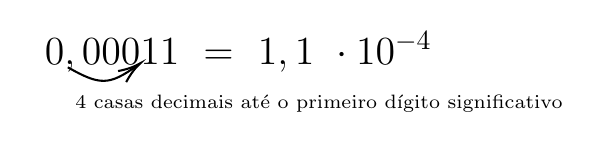
\begin{tikzpicture}[x=0.75pt,y=0.75pt,yscale=-1,xscale=1]
%uncomment if require: \path (0,71); %set diagram left start at 0, and has height of 71

%Curve Lines [id:da5246758628503831] 
\draw    (46.83,34) .. controls (62.27,42.69) and (66.54,42.99) .. (80.3,33.11) ;
\draw [shift={(81.83,32)}, rotate = 503.75] [color={rgb, 255:red, 0; green, 0; blue, 0 }  ][line width=0.75]    (10.93,-3.29) .. controls (6.95,-1.4) and (3.31,-0.3) .. (0,0) .. controls (3.31,0.3) and (6.95,1.4) .. (10.93,3.29)   ;

% Text Node
\draw (28,15.4) node [anchor=north west][inner sep=0.75pt]    {{\Large $\ 0,00011\ =\ 1,1\ \cdot 10^{-4} \ $}};
% Text Node
\draw (49,46) node [anchor=north west][inner sep=0.75pt]  [font=\scriptsize] [align=left] {4 casas decimais até o primeiro dígito significativo};


\end{tikzpicture}






\begin{center}
    \href{https://youtu.be/S22SHYt4n-o}{
        \qrcode{https://youtu.be/S22SHYt4n-o}
    }\\
    Resolução: \url{https://youtu.be/szsZ_Uuk1zk}
\end{center}
